\documentclass{article}
\usepackage[utf8]{inputenc}
\usepackage[spanish,mexico]{babel}
\usepackage[margin=2.3cm]{geometry}
\usepackage{graphicx}
\usepackage[export]{adjustbox}
\usepackage{caption}
\usepackage{subcaption}
\usepackage{fancyhdr}
\usepackage{lipsum}

% Evitar sangrías
\setlength{\parindent}{0cm}

\usepackage{amsmath}
%%\usepackage{graphicx}
%%\usepackage{subcaption}
\usepackage{amsmath}
\usepackage{amssymb}
\usepackage{amsthm}
\usepackage{url}

%%Tablas con color
\usepackage{xcolor, colortbl}
\usepackage{array, multirow, multicol}
\cellcolor[modelo color]{color}

\pagestyle{fancy}
\fancyhf{}

\title{Plantilla Facultad de Ciencias, UNAM}
\date{\today}

\begin{document}

\thispagestyle{empty}
	
	\begin{figure}[ht]
	   \minipage{0.76\textwidth}
			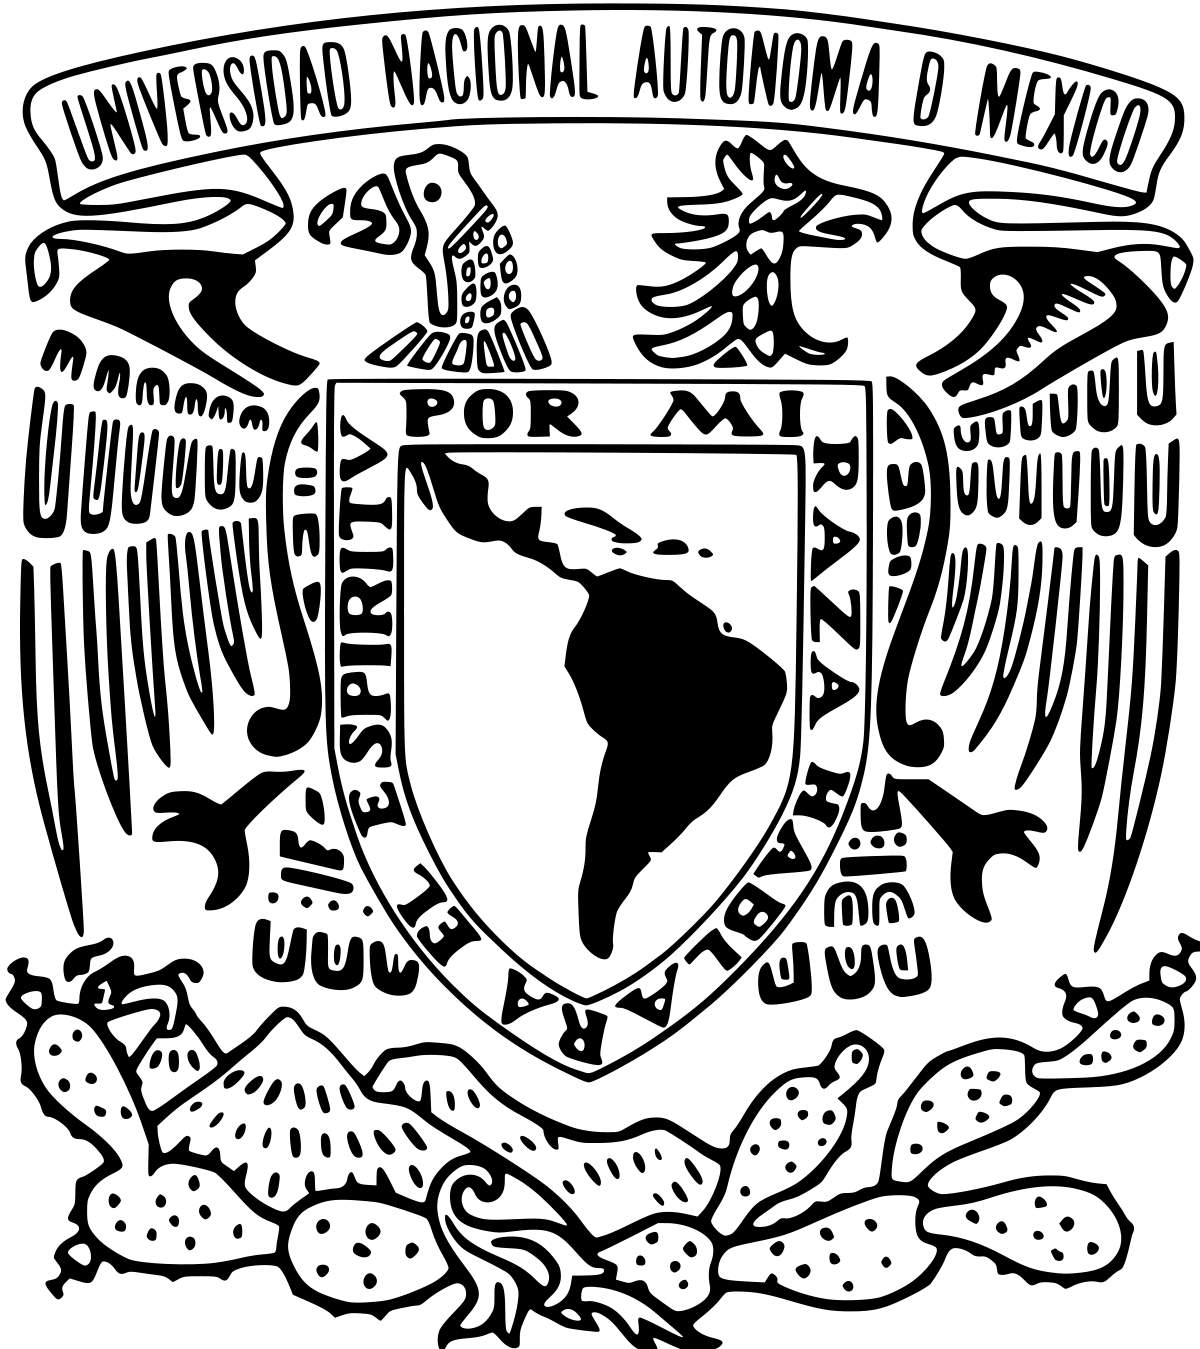
\includegraphics[width=4cm]{Logo_UNAM.png}
			\label{EscudoUNAM}
	   \endminipage
	   \minipage{0.32\textwidth}
			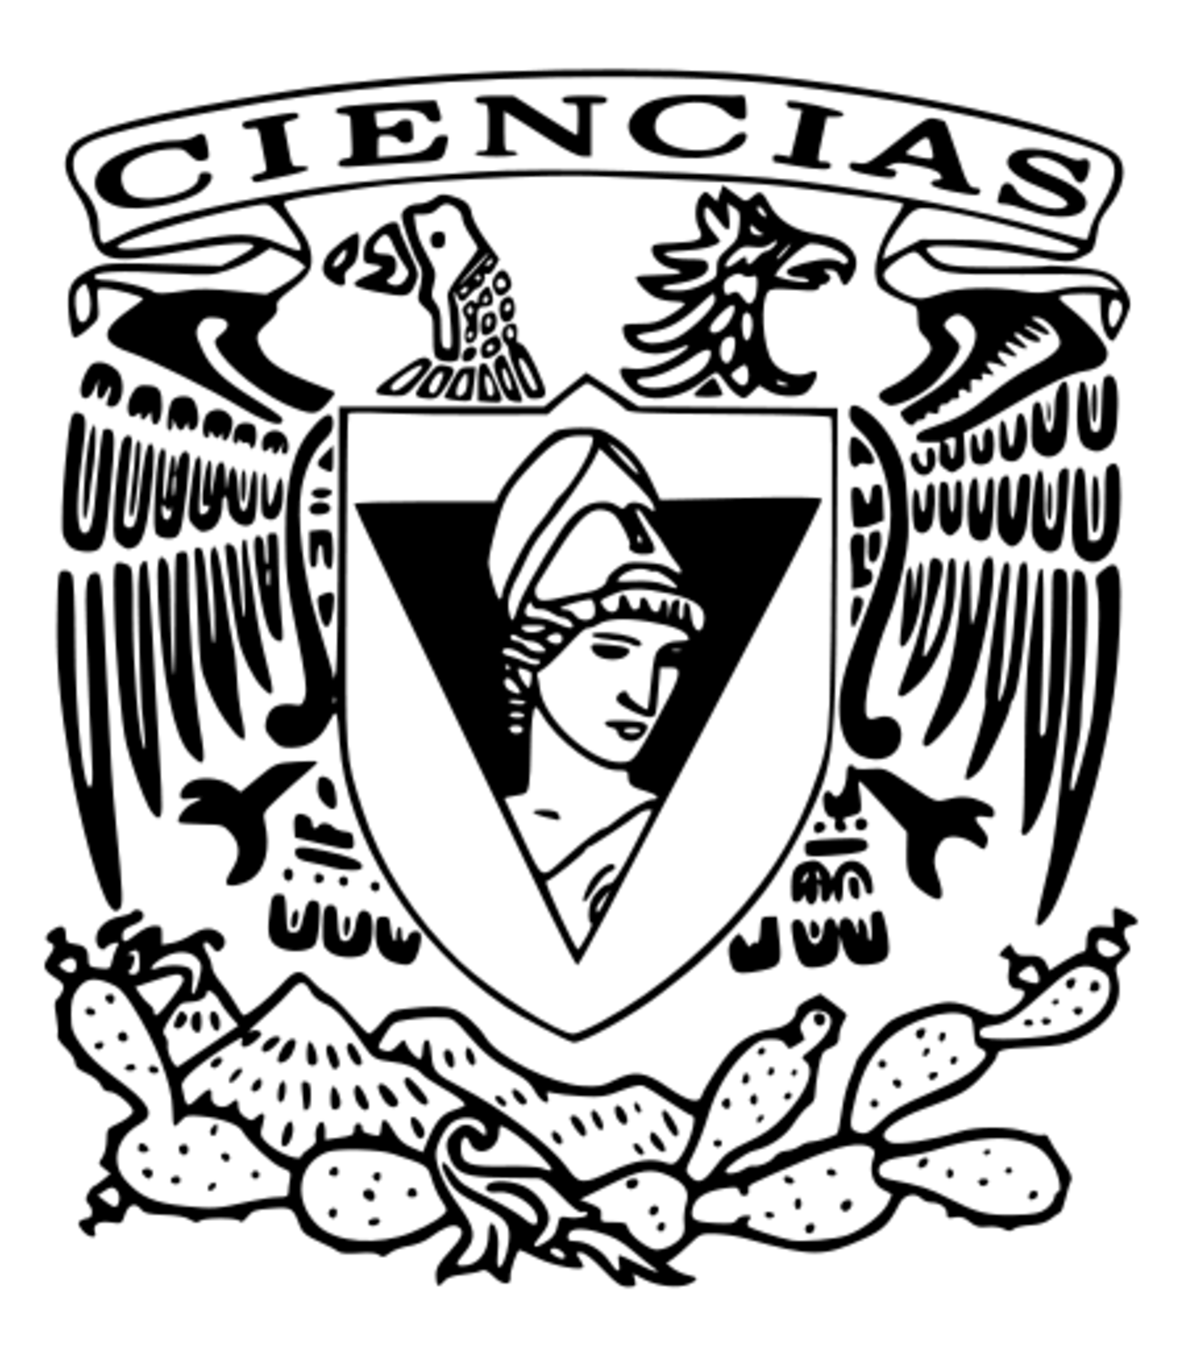
\includegraphics[height = 4.9cm ,width=4cm]{Logo_FC.png}
			\label{EscudoFC}
		\endminipage
	\end{figure}
	
	\begin{center}
	\vspace{0.8cm}
	\LARGE
	UNIVERSIDAD NACIONAL AUTÓNOMA DE MÉXICO 
	
	\vspace{0.7cm}
	\LARGE
	FACULTAD DE CIENCIAS
	
	\vspace{0.8 cm}	
	\Large
	\textbf{Tarea 1}

	\vspace{0.8 cm}
	\normalsize	
	INTEGRANTES \\
	\vspace{.2cm}
	\large
	\textbf{Torres Valencia Kevin Jair - \texttt{318331818}}\\
	\textbf{Aguilera Moreno Adrián - \texttt{421005200}}\\
	\textbf{Rivera Silva Marco Antonio - \texttt{318183583}}\\
	%\textbf{Nombre - \texttt{Número de cuenta}}
	
	\vspace{1 cm}
	\normalsize	
	PROFESORA \\
	\vspace{.2cm}
	\large
	\textbf{Karla Ramírez Pulido}
	
	\vspace{1 cm}
	AYUDANTES \\
	\vspace{.2cm}
	\large
	\textbf{Alan Alexis Martínez López}\\
	\textbf{Manuel Ignacio Castillo López}\\
	\textbf{Alejandra Cervera Taboada}
	\vspace{1.3cm}
	
	\normalsize	
	ASIGNATURA \\
	\vspace{.2cm}
	\large
	\textbf{Lenguajes de Programación}
	
	\vspace{1 cm}
	\today
	\end{center}
	
	\newpage
	\section*{Pregunta 1}
\Large 
Elige 4 lenguajes de programación (uno por cada paradigma), e indica para cada uno de ellos el año de creación, paradigma al que pertenece y principales características.\\
\newline
\large
Aqui pueden comenzar a poner sus respuestas.
\newline
Prueba de respuesta.

	\newpage
\section*{Pregunta 2}

LISP es considerado el primer lenguaje de programación funcional. Y esta basado en el Cálculo $\lambda$ que fue desarrollado por Alonzo Church.

\begin{itemize}
\item Investiga y explica brevemente qué elementos del Cálculo $\lambda$ están presentes en LISP e indica por qué crees que pueden usarse en un lenguaje de programación.

$\rhd$ Estos elementos\footnote{Cálculo $\lambda$ y LISP.} realizan
procedimientos principalmente con funciones, aunque una notable diferencia
sería que en el cálculo $\lambda$ no se trabaja con algún tipo de datos,
pues estos no existen, y en LISP tenemos tipos de datos hetereogéneos como
los atómos. Los atómos podrían biyectarse con la aplicación a términos de
una función lambda (sin embargo no son exactamente igual).

Una característica que puede ser común entre el cálculo $\lambda$ y LISP es
la recursión, pues mientras en LISP se utiliza principlamente la recursión
para operar sus funciones, en LISP se utilizan las $\beta$-reducciones

\hfill $\lhd$
\item Menciona cuáles de estos elementos están presentes en el lenguaje de programación JAVA. ¿Acaso estos elementos estaban en las primeras versiones del lenguaje? De no ser así ¿porqué crees que fueron añadidos?
\end{itemize}

    \newpage
\section*{Pregunta 3}
Describe las principales características de los distintos paradigmas
de programación (Estructurado, Orientado a Objetos, Funcional y Lógico)
y da a 2 ejemplos de lenguajes de programación de cada paradigma.

$\rhd$ Para esta pregunta, explicamos cada parádigma por separado,
esto es
\begin{center}
  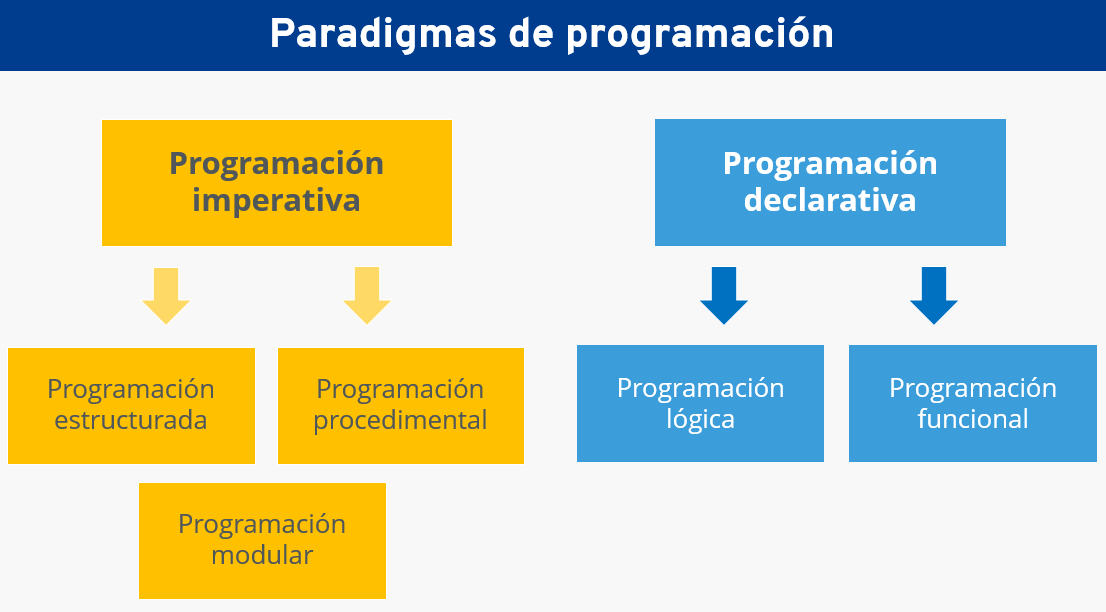
\includegraphics[scale=0.40]{./Paradigmas.png}
\end{center}

\subsection*{Parádigma Imperativo}
Describe la programación en términos del estado del programa
y sentecnias que cambian dicho estado. Se le debe explicar
el como hacer las cosas.

\begin{itemize}
\item \textbf{Orientado a objetos.}
Las principales características en las orientación a objetos
son; el polimorfismo (diseñar objetos que compartan comportamientos,
y los puedan heredar), encapsulamiento (la información referente
a un objeto esta contenida en este y puede no ser accesible al
exterior), reutilización de código (modularizar nos permite evitar
duplicar código), los conceptos de clases y objetos (nuestros
objetos tendrán comportamientos definidos en clases).

Ejemplos de lenguajes orientados a objetos:
\begin{enumerate}
\item C++.
\item JAVA.
\end{enumerate}
\item \textbf{Estructurado.}
Las principales características en los lenguajes estructurados
son; la sintaxis (orden y reglas del lenguaje), la semántica
(interpretación y significado de la sintaxis), la pragmática
(modo en que el contexto o situación le entrega interpretación
al significado).

Ejemplos de lenguajes estructurados:
\begin{enumerate}
\item C.
\item PASCAL.
\end{enumerate}
\end{itemize}
\subsection*{Parádigma Declarativo}
Este paradigma de programación esta basado en el desarrollo de
programas ``declarando'' un conjunto de condiciones, proposiciones,
afirmaciones, restricciones, ecuaciones o transformaciones que
describen el que requiera y no el como hacer.

\begin{itemize}
\item \textbf{Funcional.}
Las principales características de la programación funcional
son; semántica limpia (no hay ambigüedades en el significado
de las funciones, almacenamiento implícito de datos),
inexistencia de efectos colaterales (no hay asignación a
variables globales), utilización del cálculo-$\lambda$ (independencia
fuera de la función).

Ejemplos de lenguajes funcionales:
\begin{enumerate}
\item Racket.
\item Haskell.
\end{enumerate}
\item \textbf{Lógico.}
Las principales características de los lenguajes en el paradigma lógico
son; reglas (conjunto de proposiciones lógicas escritas como clausulas
de Horn), hechos (Expresiones atómicas que verifican un predicado sobre
algunos entes que puede procesar el mismo), consultas (proposiciones
que se verifican para algún valor de verdad), recursión.

Ejemplos de lenguajes lógicos:
\begin{enumerate}
\item GODEL.
\item PROLOG.
\end{enumerate}
\end{itemize}
\hfill $\lhd$

	\newpage
\section*{Pregunta 4}
\Large 
¿Cuál de los paradigmas de lenguajes de programación, es el más adecuado para resolver los siguientes problemas? Justifica en cada caso.\\\\
%%%%%%%%%%%%%%%%%%%%%%%%%%%%%%%%%%%%%%%%%%%%%%%%%%%%%%%%%
a) Se requiere desarrollar un sistema que simule un modelo de sociedad de organización de termitas. Este sistema se compone, de manera general de: un espacio que las termitas recorrerán y en el cuál se encuentran astillas esparcidas, las termitas siguen las siguientes reglas de comportamiento.\\
\begin{itemize}
\item Caminan aleatoriamente hasta encontrar una astilla.
\item Si la termita se encuentra cargando una astilla, la suelta y continúa caminando aleatoriamente.
\item Si la termita no está cargando una astilla la toma y continúa caminado aleatoriamente con la astilla
\end{itemize}
\large
Aqui pueden comenzar a poner sus respuestas.\\


	\newpage
%\section*{Pregunta 4b}
\Large
b) El Problema de las Ocho Reinas consiste en acomodar ocho reinas de ajedrez en un tablero, sin que ninguna de éstas se ataque entre sí. Una reina, puede atacar (a) de forma vertical, (b) de forma horizontal y (c) en diagonal. Usando estas reglas, indicar si el siguiente tablero es una solución al problema de las ocho reinas.\\

\begin{figure}[h!]
\centering
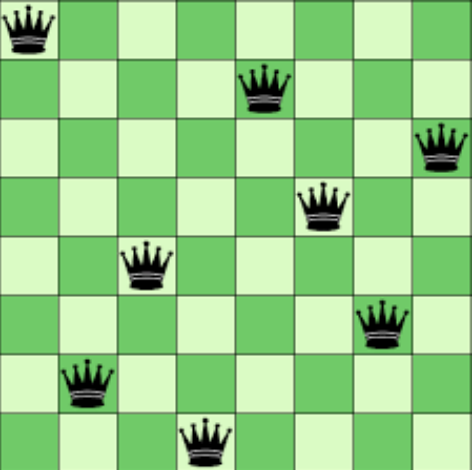
\includegraphics[scale=0.35]{Tablero.png}
\end{figure}
\large
Aqui pueden comenzar a poner sus respuestas.\\
	\newpage
%\section*{Pregunta 4c}
\Large
c) Escribir un programa que indique si un número natural es primo. Un número es primo.\\
\newline
\large
Aqui pueden comenzar a poner sus respuestas.\\
	%\section*{Pregunta 4d}
\Large

d) Dado un archivo con los primeros 10,000 dígitos de $\pi$, contar todas las apariciones de números primos presentes en él.\\
\newline
\large

Debido al tamaño de la entrada, determinamos que la mejor opción es una busqueda con un lenguaje de programación imperativa, pues
se puede controlar mejor la busqueda con iteraciones, además de que no tenemos que preocuparnos por la pila de ejecución. Para este caso
puede ser mejor el estructurado sobre el orientado a objetos ya que no tenemos la necesidad de usar objetos (considerando que no tenemos que importar el archivo como objeto).
	\newpage
\section*{Pregunta 5}
\Large
Investiga que significan los siguientes conceptos en un lenguaje de programación. Y elabora un pequeño ejemplo ocupando como base al lenguaje de programación HASKELL.\\\\
%%%%%%%%%%%%%%%%%%%%%%%%%%%%%%%%%%%%%%%%%%%%%%%%%%%%%%%
a) Sintaxis.\\
\newline
\large
Aqui pueden comenzar a poner sus respuestas.\\
%%%%%%%%%%%%%%%%%%%%%%%%%%%%%%%%%%%%%%%%%%%%%%%%%%%%%%%
\newline
\Large
b) Semántica.\\
\newline
\large
Aqui pueden comenzar a poner sus respuestas.\\
%%%%%%%%%%%%%%%%%%%%%%%%%%%%%%%%%%%%%%%%%%%%%%%%%%%%%%%
\newline
\Large
c) Idioms (Convenciones de programación).\\
\newline
\large
Aqui pueden comenzar a poner sus respuestas.\\
%%%%%%%%%%%%%%%%%%%%%%%%%%%%%%%%%%%%%%%%%%%%%%%%%%%%%%%%
\newline
\Large
d) Bibliotecas.\\
\newline
\large
Aqui pueden comenzar a poner sus respuestas.\\

	\newpage
\section*{Pregunta 6}
\Large 
A partir de la siguiente función, crea una firma indicando el tipo de entrada que recibirá la función y el tipo de salida que se obtendrá de la función. Asigna un nombre mnemotécnico (es decir que se autodescriba) para la misma. Justifica tu respuesta.

\large
\begin{verbatim}
(define (foo a b)
(cond
[(> (car a) (car b)) (sub1 (foo (cdr a) (cdr b)))]
[else 0]))
\end{verbatim}
%%%%%%%%%%%%%%%%%%%%%%%%%%%%%%%%%%%%%%%%%%%%%%%%%%%
\large
La funcion recibe dos pairs (a y b) y recursivamente va comparando entre la cabezas de ambos pairs, hasta obtener que a $\leq$ b, reduciendo el indice de los elementos del pair (cola) hasta que este sea negativo. De lo contrario arrojara 0 por automático.

\large
\begin{verbatim}
	;; Funcion que recibe dos pairs y regresa su menor indice.  
	;; menor-indice-del-elemento-pequeño: (pair a) (pair b) -> number
\end{verbatim}
	\newpage
\section*{Pregunta 7}
\Large 
Calcula el resultado de las siguientes funciones en el lenguaje de programación Racket y muéstralo. Posteriormente realiza tu propia implementación de cada función.\\\\
%%%%%%%%%%%%%%%%%%%%%%%%%%%%%%%%%%%%%%%%%%%%%%%%%%%%%%%%%%%%%%%
a) (second '(1 7 9 4 5 6))\\
\newline
\large
Aqui pueden comenzar a poner sus respuestas.\\
%%%%%%%%%%%%%%%%%%%%%%%%%%%%%%%%%%%%%%%%%%%%%%%%%%%%%%%%%%%%%%%
\newline
\Large
b) (append ’(Bue) ’(n semestre))\\
\newline
\large
Aqui pueden comenzar a poner sus respuestas.
	\newpage
\section*{Pregunta 8}
\Large 
Dibuja un mapa mental que muestre las fases de generación código ejecutable, sus principales características y elementos involucrados..\\
\newline
\large
\begin{figure}[h!]
	\centering
	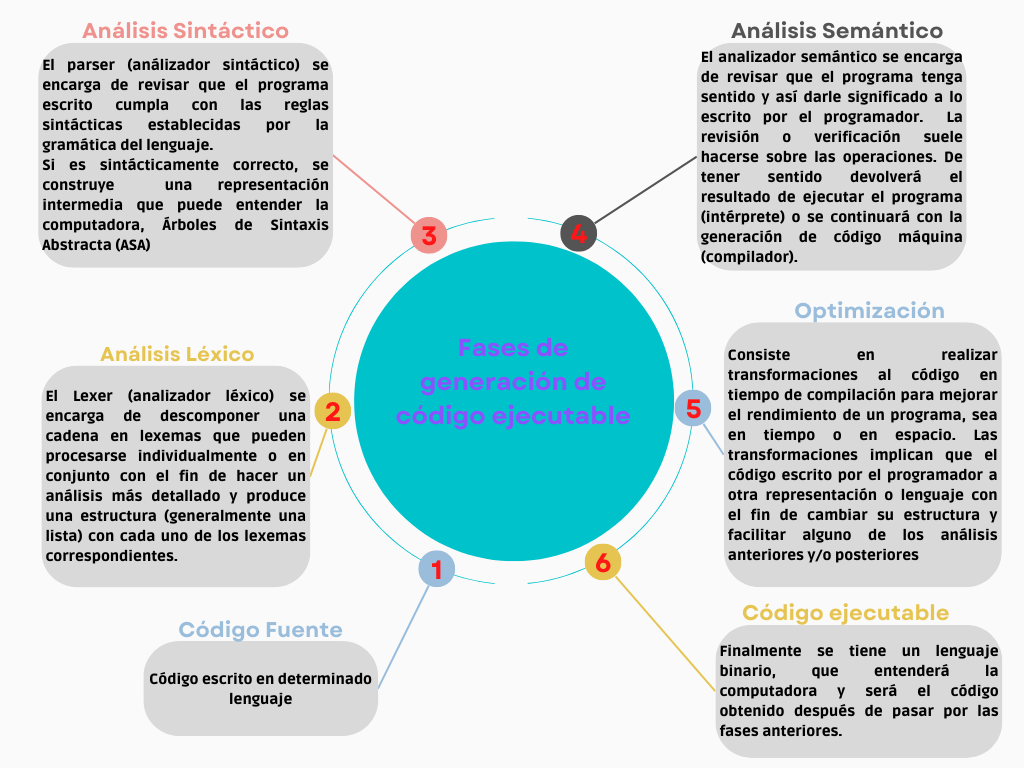
\includegraphics[scale=0.71]{Mapa.png}
\end{figure}
\end{document}
